\section{Data}

\textit{Uppsala Conflict Data program} samler inn og verifiserer data om
konflikter og organisert vold i hele verden. Et av datasettene,
\textit{Georeferenced Event Dataset (GED)} består av dødsfall som et resultat
av organisert vold. Organisert vold er i denne sammenhengen hendelser i en
konflikt som har resultert i dødsfall, og hvor minst en part i konflikten er en
organisert enhet. Hvert datapunkt i GED er definert som en hendelse. For at en
hendelse skal bli inkludert i datasettet må det ha skjedd minst et verifisert
dødsfall. Dataene blir samlet inn fra nyhetskilder, rapporter fra forskjellige
autoriteter og organisasjoner, og blir forsøkt verifisert fra flere kilder.
Tidspunkt og sted for hendelsene blir estimert med størst mulig nøyaktighet.
Informasjon om parter i konflikten blir også fastsatt. Datasettet starter med
hendelser fra 01.01.1989 og strekker seg fram til 31.12.2021. 


\begin{table}[!h]
\centering

\begin{tabular}[t]{llrrrrr}
\toprule
date\_start & country & date\_prec & type\_of\_violence & best & high & low\\
\midrule
2017-07-31 & Afghanistan & 1 & 1 & 6 & 6 & 6\\
2021-08-26 & Afghanistan & 1 & 1 & 183 & 184 & 171\\
2021-08-28 & Afghanistan & 1 & 1 & 2 & 3 & 0\\
$\vdots$ & $\vdots$ & $\vdots$ & $\vdots$ & $\vdots$ & $\vdots$ & $\vdots$ \\ 
 \bottomrule
\end{tabular}
\caption{De første radene i GED-datesettet. Variabler som ikke er relevante for
denne oppgaven er utelatt.}
\label{tab:GED_table}
\end{table}

Vi skal se på ukentlige antall dødsfall som resultat av organisert vold. Det
har vi definert som hendelser hvor staten er en aktør i konflikten. Hendelser i
konflikter mellom to ikke statlige aktører ble filtrert ut. Videre brukte vi
det beste estimatet for antall døde. Hendelser hvor tidspunktet ikke kunne
bestemmes mer nøyaktig enn på måned eller år, ble utelatt. Land med færre enn
100 uker med hendelser ble også utelatt. Antall dødsfall ble så aggregert for
hver uke i hvert land. For antall dødsfall pr hendelse bruker vi det beste
estimatet. I den endelige undersøkelsen endte vi opp med datasett med tre
variabler: uke, land og antall døde. Det vil si for hvert land har vi en
tidsserie med antall dødsfall pr uke mellom 01.01.1989 til 31.12.2021. Land med
færre enn 100 uker med hendelser ikke inkludert.

For å kvantifisere graden av overspredning av dødsfall for hvert land kan man
sammenligne den observerte fordelingen med en teoretisk poisson-fordeling med
samme forventning som de observerte dataene \parencite{weiss2018introduction}.
Dette gir opphav til  spredningsindeksen $I_{\mathrm{disp}}$. Gitt det
observerte gjennomsnittet $\hat{\mu}$ og den observerte variansen
$\hat{\sigma}^2$ blir 

 $$
    I_{\mathrm{disp}} = \frac{\hat{\sigma}^2}{\hat{\mu}}.
 $$

Ved $I_{\mathrm{disp}} = 1$ er variansen lik gjennomsnittet, noe som er
karakteristisk for poissonfordelingen. Er $I_{\mathrm{disp}} < 1$ har dataene
underspredning: I motsatt tilfelle når $I_{\mathrm{disp}} > 1$ har dataene
overspredning. 

Andelen 0-verdier ble brukt direkte som et mål for zero-inflation:

$$
\hat{p_0} = \frac{1}{N}\sum_{t=1}^N \mathds{1}(Y_{i,t}=0).
$$

    \begin{figure}[!h]
    \centering
    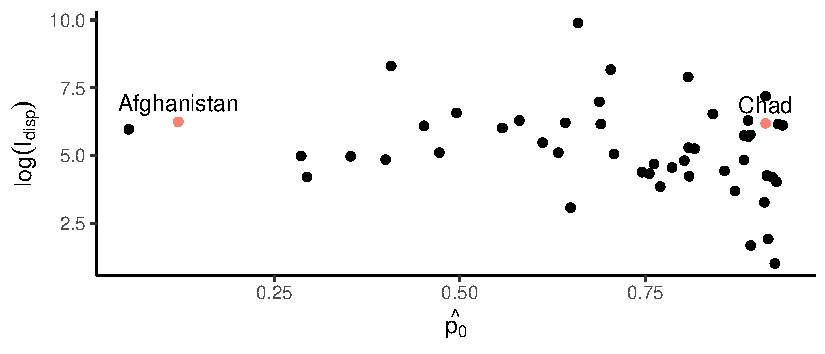
\includegraphics{../img/index_plot.pdf}
        \caption{
            Logaritmen til $I_{\mathrm{disp}}$ og andel 0-verdier ($\hat{p_0}$) for
            de inkluderte landene. Chad og Afghanistan er uthevet.
        }
    \label{fig:index_plot}
    \end{figure}

I \cref{fig:index_plot} vises en oppsummering av spredningsindeksen og andelen
0-verdier for alle landene som er inkludert. Afghanistan og Chad har omtrent
samme spredningsindeks, men er i hver ende av skalaen for andelen 0-verdier.

